\documentclass[11pt,letterpaper]{article}
\usepackage[T1]{fontenc}
\usepackage{mathptmx}
\usepackage[margin=1in]{geometry}
\usepackage{amsmath,amssymb}
\usepackage{booktabs,tabularx}
\usepackage{enumitem}
\usepackage{tikz}
\usetikzlibrary{arrows.meta,positioning,fit,calc,backgrounds,shapes.geometric}
\usepackage[font=small,labelfont=bf,textfont=it]{caption}
\usepackage{url}
\usepackage{xurl}
\emergencystretch=3em
\usepackage[hidelinks]{hyperref}
\usepackage{titlesec}
\titleformat{\section}{\normalfont\large\bfseries}{\thesection.}{0.5em}{}
\titleformat{\subsection}{\normalfont\normalsize\bfseries}{\thesubsection}{0.5em}{}
\setlength{\parindent}{1.5em}
\setlength{\parskip}{2pt}
\renewcommand{\arraystretch}{1.15}

\newcommand{\authorname}{Thor Thor}
\newcommand{\orcidid}{0009-0001-6573-385X}

\usepackage{amsthm}
\theoremstyle{definition}
\newtheorem{definition}{Definition}
\newtheorem{proposition}{Proposition}

% notation
\newcommand{\St}{\Sigma}
\newcommand{\Inv}{\Gamma}
\newcommand{\Pre}{\mathrm{Pre}}
\newcommand{\Add}{\mathrm{Add}}
\newcommand{\Del}{\mathrm{Del}}
\newcommand{\Next}{\mathrm{Next}}
\newcommand{\En}{\mathrm{Enabled}}
\newcommand{\Ap}{\mathrm{Apply}}
\newcommand{\End}{\mathrm{End}}
\newcommand{\Lang}{\mathcal{L}}
\newcommand{\Fam}{\mathcal{F}}
\newcommand{\Mod}{\mathcal{M}}
\newcommand{\Comp}{\mathrm{Compromise}}
\newcommand{\evsep}{\mathrel{\vdots}}

\tikzset{
  box/.style={draw, rectangle, rounded corners=1.5pt, align=center, font=\sffamily\scriptsize, minimum height=8mm, inner sep=3pt, fill=white},
  ebox/.style={draw, rectangle, dashed, align=center, font=\sffamily\scriptsize, minimum height=8mm, inner sep=3pt, fill=white},
  arr/.style={-{Stealth[length=2mm]}, semithick},
  darr/.style={-{Stealth[length=2mm]}, semithick, dashed},
  lbl/.style={font=\sffamily\tiny, fill=white, inner sep=1pt},
  capn/.style={font=\sffamily\scriptsize\itshape, align=center},
  st/.style={draw, circle, minimum size=7mm, inner sep=0pt, font=\sffamily\scriptsize},
  goal/.style={draw, circle, double, minimum size=7mm, inner sep=0pt, font=\sffamily\scriptsize},
}

\hypersetup{pdftitle={Attack Calculus: A Typed, Evidence-Aware State-Transition Calculus for Cross-Domain Cybersecurity Reasoning}, pdfauthor={Thor Thor}}

\begin{document}

\begin{center}
{\LARGE\bfseries Attack Calculus: A Typed, Evidence-Aware State-Transition Calculus for Cross-Domain Cybersecurity Reasoning\par}
\vspace{0.6em}
{\large Formal Semantics, Evidence-Consistent Models, Robust Defensive Synthesis, and an AI-Agent Extension\par}
\vspace{1.0em}
{\large \authorname\par}
\vspace{0.3em}
{\small Independent Open-Source Researcher, THOR-SEC\\
ORCID: \href{https://orcid.org/\orcidid}{\orcidid} \quad \url{codethor@gmail.com}\\
GitHub: \url{https://github.com/codethor0} \quad \url{https://codethor0.github.io/thor-sec/}\par}
\vspace{0.3em}
{\small This research was conducted independently on the author's own time and is not sponsored by, affiliated with, or representative of any employer.\par}
\vspace{0.3em}
{\small Preprint, October 2026. Released openly for community review.\par}
\end{center}

\begin{abstract}
\noindent Cybersecurity frameworks classify adversary behavior, exchange threat intelligence, catalog defensive techniques, and generate attack graphs, yet incident reasoning still lacks a compact notation that states at once why an action occurs, how it occurs, which state enables it, which state it changes, and what evidence supports each claim. This paper proposes Attack Calculus Notation (ACN), a typed, evidence-aware state-transition calculus that connects analyst-readable incident reasoning to machine-checkable models. Each atomic action is an actor-labelled transition with explicit intent, mechanism, target, object, channel, valued guards, add and delete effects, and field-level evidence. Compact expressions denote finite trace languages and compile to a guarded predicate-transition model equivalent to typed STRIPS planning, which fixes the complexity of compromise checking. Evidence uncertainty defines a family of admissible models, over which ACN distinguishes possible from necessary compromise. Defensive controls are model transformations, and robust task-preserving synthesis selects the least-cost control bundle that eliminates every modeled prohibited outcome in every admissible model while keeping authorized-task utility above a floor in the worst admissible model. An AI-agent extension separates influence from authority and measures excess authority with a capability subsumption order. A complete worked example, reproduced by a published reference checker, shows a case where an analysis restricted to the most likely model selects a control that fails in an admissible alternative, and where attack-only minimization breaks a business task. The work is a formal specification and falsifiable research program; it claims no empirical superiority.
\end{abstract}
\vspace{-0.4em}
\noindent\textbf{Keywords:} attack modeling; state transitions; automated planning; evidence provenance; formal methods; defensive synthesis; least privilege; AI-agent security; incident reasoning
\medskip

\section{Introduction}

Security analysis often begins with labels such as ransomware, phishing, identity compromise, prompt injection, supply-chain compromise, or process manipulation. These labels are useful for communication, but they do not determine execution logic. Two incidents with the same label may depend on different credentials, trust assumptions, channels, privilege transitions, reachable resources, or defensive failures. The central object of analysis is therefore not the attack name but the state transformation that makes the next action possible.

Attack Calculus begins from a simple premise: an attack is a sequence, branch, loop, or partially ordered set of state transformations. The useful unit of reasoning is an atomic transition with explicit prerequisites and effects. The notation is intended to be readable by incident responders and threat analysts, structured enough for parsers, and constrained enough that unsupported prerequisites and contradictory effects are detected mechanically.

The problem is not a lack of formal models. Attacks have been described by preconditions and postconditions since LAMBDA and the requires/provides model of JIGSAW \cite{cuppens2000,templeton2000}, and as state transitions for intrusion detection since STATL \cite{statl}. Alert correlation has linked attack steps through prerequisites and consequences \cite{ning2002}. Attack graphs have been generated by model checking and by logic programming \cite{sheyner2002,ammann2002,mulval}, attack-defense trees provide goal decomposition with attacker-defender semantics \cite{adtrees}, and the Meta Attack Language generates attack graphs from domain models \cite{mal,konsta2024}. Automated planning has been used to generate attack courses of action and to simulate penetration testing \cite{boddy2005,obes2010,hoffmann2015}. ATT\&CK supplies a behavioral taxonomy, D3FEND a countermeasure knowledge graph, and STIX an exchange format \cite{attack,d3fend,stix}.

The narrower research question is whether a single analyst-facing intermediate representation can preserve causal execution logic and epistemic evidence while compiling to machine-checkable models that interoperate with these taxonomies. The working hypothesis is that such a representation makes disagreements inspectable, exposes missing prerequisites, keeps reconstruction from silently becoming fact, and connects incident reasoning to defensive synthesis without requiring analysts to author a full formal model.

ACN makes five proposed contributions: (1) a typed atomic transition with valued guards, additive and destructive effects, and field-level evidence; (2) a composition grammar with denotational trace semantics; (3) evidence-consistent model families with possible and necessary compromise; (4) robust task-preserving defensive synthesis with worst-case utility; and (5) a subsumption-aware measure of excess agent authority. A worked example in Section~\ref{sec:example} exercises every definition with computed values, and a reference checker reproduces them.

\section{Research Position and Relation to Prior Work}\label{sec:related}

A credible calculus must state what it does not invent. Table~\ref{tab:position} summarizes the position; this section gives the reasoning.

\paragraph{Precondition-effect attack languages.} LAMBDA specified attacks by pre-condition, post-condition, scenario, detection, and verification \cite{cuppens2000}. JIGSAW modeled attacks through capabilities each step requires and provides \cite{templeton2000}. Ning, Cui, and Reeves correlated alerts by matching consequences to prerequisites \cite{ning2002}. STATL describes intrusion scenarios as state transitions \cite{statl}. ACN inherits this precondition-effect view. Its differences are explicit delete effects, explicit negative values, field-level evidence status, and a defined trace semantics for composition.

\paragraph{Attack graphs and monotonicity.} Model-checking attack graphs \cite{sheyner2002}, scalable graph-based vulnerability analysis \cite{ammann2002}, and MulVAL \cite{mulval} established automated attack-graph generation. The scalable approaches rely on a monotonicity assumption: an attacker never loses a capability once gained. That assumption is what makes them tractable, and it is also what ACN deliberately drops. Credential rotation, session termination, isolation, recovery, and defense impairment all remove facts. ACN therefore trades the polynomial guarantees of monotone analysis for the ability to represent these reversals, and states the resulting complexity in Section~\ref{sec:complexity}.

\paragraph{Automated planning.} A ground ACN model with valued atoms, preconditions, add effects, and delete effects is a typed STRIPS planning task \cite{strips,pddl}, and model-relative compromise is plan existence. Planning has been applied to attack generation and penetration testing \cite{boddy2005,obes2010,hoffmann2015}. This connection is a strength rather than a threat to the contribution: it imports known complexity results \cite{bylander1994}, mature solvers, and a precise vocabulary. ACN's additions to plain planning are evidence objects and evidence-consistent model families, possible versus necessary compromise, the analyst-facing compact syntax, and synthesis that preserves authorized tasks across the family.

\paragraph{Concurrency and nets.} The compiled object resembles a predicate/transition net \cite{genrich1981}, and the independence relation of Section~\ref{sec:conc} is the standard independence of Mazurkiewicz trace theory and partial-order reduction \cite{mazurkiewicz1987,godefroid1996}, used here only as a conservative admission rule.

\paragraph{Defensive optimization.} Network interdiction and resource-constrained optimization over attack graphs predate ACN \cite{nandi2016,bhuiyan2021}. Neither state-transition modeling, attack-graph generation, planning-based attack analysis, nor finding a cut set is claimed as new. Structural defenses that change the model itself, such as service-graph morphing across security epochs \cite{miam}, fit Definition~\ref{def:control} as model transformations.

\paragraph{AI-agent security.} Prompt injection manipulates agent behavior through attacker-controlled content \cite{openai2025,toolhijacker}. Task Shield checks each action against the user's task \cite{taskshield}. CaMeL separates trusted control flow from untrusted data with capability restrictions \cite{camel}, and Progent enforces deterministic privilege policies on tool calls \cite{progent}. Vendor guidance recommends constraining the consequences of manipulation \cite{openai2026} and scoping agent identity, resources, and tools \cite{microsoft2026}. AuthGraph compares an authorization graph against execution provenance \cite{authgraph}, reachability-based confinement recomputes capability restrictions after contamination \cite{xiong2026}, and SkillGuard treats agent skills as permission-bearing artifacts \cite{skillguard}. The confinement system of \cite{xiong2026} is also named SkillGuard; the two are unrelated. ACN does not propose a new authorization primitive. It expresses influence, delegated authority, tool scope, resource reachability, and egress in the same transition semantics used for other domains, so that agent incidents and conventional incidents are analyzed with one model.

\begin{table}[t]
\centering\small
\caption{Positioning of ACN relative to established work.}\label{tab:position}
\begin{tabularx}{\textwidth}{@{}l l X@{}}
\toprule
System & Primary role & ACN position \\
\midrule
LAMBDA, JIGSAW, STATL & Pre/post attack specification & ACN inherits pre/post transitions; adds delete effects, valued negatives, evidence, and trace semantics. \\
MulVAL and monotone attack graphs & Scalable attack-graph generation & ACN drops monotonicity to represent revocation and recovery, at a stated complexity cost. \\
STRIPS, PDDL, attack planning & Plan existence and generation & ACN models compile to typed STRIPS; ACN adds evidence families and task-preserving synthesis. \\
Attack-defense trees, MAL & Goal decomposition, domain DSL & ACN is trace and incident oriented; interoperation is preferable to duplication. \\
ATT\&CK, D3FEND, STIX & Taxonomy, countermeasures, exchange & External mappings remain metadata; guards, effects, and evidence are ACN semantics. \\
CaMeL, Progent, AuthGraph & Agent authorization and provenance & ACN models these controls as transformations in a shared cross-domain semantics. \\
\bottomrule
\end{tabularx}
\end{table}

\section{Formal Objects}\label{sec:formal}

\subsection{Typed state, values, and invariants}

Let $\mathcal{S}$ be an extensible set of sorts, such as Actor, Principal, Asset, Process, Credential, Token, Resource, Channel, Capability, Tool, Policy, Data, and PhysicalState. Each predicate symbol $p$ has a signature $\mathrm{sig}(p)=(s_1,\dots,s_n;V_p)$, where $V_p$ is a finite value domain. A ground atom $p(v_1,\dots,v_n)=u$ is well typed exactly when each $v_i$ has sort $s_i$ and $u\in V_p$:
\begin{equation}
\Delta\vdash p(v_1,\dots,v_n)=u : \mathrm{Atom}\iff \mathrm{type}(v_i)=s_i\ \forall i \ \wedge\ u\in V_p,
\end{equation}
where $\Delta$ is the declared type environment. Boolean predicates use $V_p=\{\mathrm{true},\mathrm{false}\}$, and the shorthand $p(\vec v)$ means $p(\vec v)=\mathrm{true}$.

Let $\mathrm{Atoms}$ be the universe of well-typed ground atoms and $\Inv$ a set of domain invariants. A state $\St$ is a subset of $\mathrm{Atoms}$ that satisfies $\Inv$. $\Inv$ always includes value exclusivity: for each predicate instance $p(\vec v)$, at most one value is present. Negation-as-failure is not part of guard semantics. A guard that requires a negative condition uses an explicit value, such as $\mathrm{AUTHZ}(A,j)=\mathrm{denied}$, so that an unmodeled fact is never read as false. Uncertainty about which concrete state is correct is handled by the model families of Section~\ref{sec:evidence}.

The atom universe is partitioned into typed namespaces for knowledge, privilege, trust, control, reachability, persistence, data possession, integrity, and availability, written $N_K,\dots,N_{Av}$. The familiar nine-component view is a projection of the same set-valued state, not a second object:
\begin{equation}
\St \equiv \langle K,P,T\!r,C,R,P\!s,D\!t,I,Av\rangle,\qquad K=\St\cap N_K,\ \dots,\ Av=\St\cap N_{Av}.
\end{equation}
Domain extensions add disjoint namespaces, and $\Inv$ may constrain atoms across namespaces. Representative atoms include $\mathrm{KNOW}(A,\mathit{cred})$, $\mathrm{PRIV}(A,h)=\mathrm{admin}$, $\mathrm{TRUST}(\mathit{tok},\mathit{svc})=\mathrm{valid}$, $\mathrm{REACH}(h_1,h_2)$, $\mathrm{PERSIST}(x,h)$, $\mathrm{POSSESS}(A,f)$, $\mathrm{INTEGRITY}(r)=\mathrm{valid}$, and $\mathrm{AVAILABLE}(s)$.

\subsection{Atomic transitions, principals, and binding}

\begin{definition}[Atomic ACN transition]\label{def:atomic}
An atomic transition $\tau$ is a tuple $\langle a,b,i,m,y,x,\chi,\Pre,\Add,\Del,e\rangle$, where $a$ is the executing principal; $b$ is an optional influencing principal on whose behalf or under whose influence $a$ acts; $i$ is the intent; $m$ the mechanism; $y$ the target; $x$ the acted-upon object; $\chi$ the channel; $\Pre$, $\Add$, and $\Del$ are finite sets of typed atoms; and $e$ is an evidence object. A well-formed transition has $\Add(\tau)\cap\Del(\tau)=\emptyset$ and all fields type-correct.
\end{definition}
The compact form is
\begin{equation}
a\,[\triangleleft\, b]\ \vdash\ [\,i\mid m\,]\ y(x)\ @\ \chi\ :\ \Pre\ \Rightarrow\ (\Add,\Del)\ \evsep\ e .
\end{equation}
The influencing principal matters whenever the actor that executes an action is not the party responsible for it: an AI agent acting on injected content, a deputy misused by a caller, or a script run by a phished user. Keeping both principals avoids two errors: attributing an agent's action to the attacker as if the attacker held the agent's authority, and attributing it to the agent as if no attacker were involved.

Authoring templates may contain typed variables, but executable transitions are ground. A type-preserving substitution $\theta$ binds every variable consistently across all fields:
\begin{equation}
\mathrm{Ground}(\tau,\theta)\ \text{defined}\iff \theta\ \text{is type-preserving and binds every variable of}\ \tau .
\end{equation}
The turnstile denotes an asserted transition under stated conditions. It is not a claim that the expression is a deductive proof about the real world.

\subsection{Enablement, application, and invariant timing}

\begin{definition}[Raw successor]
For a well-formed ground transition, the candidate successor removes all delete effects and then inserts all add effects as one atomic update. The intermediate delete-only state is not observable and need not satisfy $\Inv$:
\begin{equation}\label{eq:next}
\Next(\St,\tau)=(\St\setminus\Del(\tau))\cup\Add(\tau).
\end{equation}
\end{definition}

\begin{definition}[Enablement]
A transition is enabled exactly when every guard atom is present and the complete candidate successor satisfies $\Inv$:
\begin{equation}\label{eq:enabled}
\En(\tau,\St)\iff \Pre(\tau)\subseteq\St\ \wedge\ \Next(\St,\tau)\models\Inv .
\end{equation}
A candidate that violates $\Inv$ is not executable, and a validator reports it as an invariant violation.
\end{definition}

\begin{definition}[Application]
Application is defined on the enabled domain and returns the validated successor:
\begin{equation}\label{eq:apply}
\Ap(\St,\tau)=\Next(\St,\tau)\quad\text{for}\ \En(\tau,\St).
\end{equation}
\end{definition}
Delete effects are essential. Credential rotation invalidates prior trust, isolation removes reachability, recovery removes persistence, and defense impairment removes a control's availability. A model that only accumulates facts cannot represent these reversals soundly.

\subsection{Evidence objects}\label{sec:evobj}

\begin{definition}[Evidence object]
An evidence object is
\[e=\langle \mathit{status},\ \mathit{confidence},\ \mathit{method},\ \mathit{provenance},\ \mathit{time},\ \mathit{support}\rangle,\]
where $\mathit{status}\in\{\mathrm{O},\mathrm{C},\mathrm{R},\mathrm{U}\}$ (observed, corroborated, reconstructed, unresolved); $\mathit{confidence}$ is optional and requires a declared calibration $\mathit{method}$; $\mathit{provenance}$ identifies source material; $\mathit{time}$ is a timestamp or interval; and $\mathit{support}\subseteq\{\text{occurrence},\text{guard},\text{add\_effect},\text{delete\_effect},\text{ordering},\text{mapping}\}$. Every transition carries an evidence object, and so does every atom of the initial state $\St_0$.
\end{definition}
Field-level support allows evidence to establish that an event occurred without establishing the analyst's reconstructed guard. Attaching evidence to initial atoms closes a gap in which a trace could rest on an initial fact with no recorded basis. Evidence status is categorical metadata, not a probability, and does not change execution. ACN forbids deriving confidence by assigning fixed numbers to O, C, R, and U. Provenance records may be serialized with W3C PROV \cite{prov}.

\begin{figure}[t]
\centering
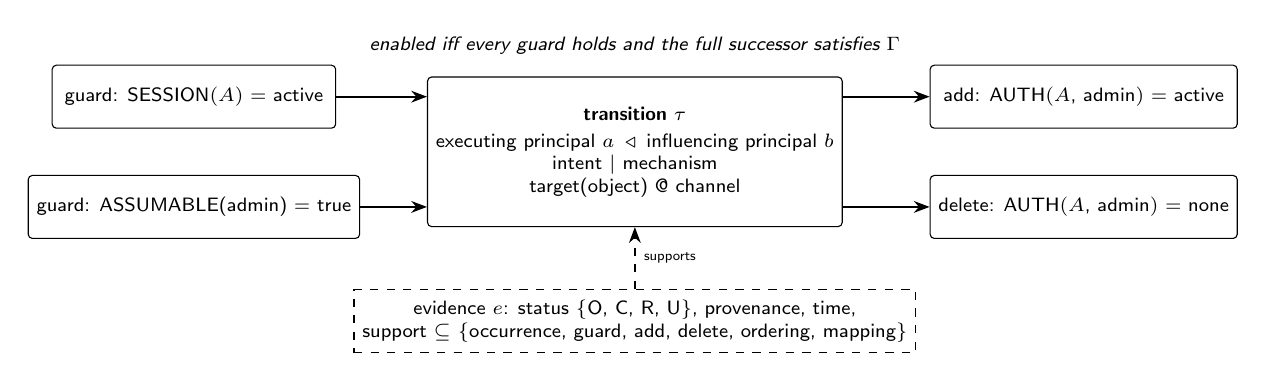
\begin{tikzpicture}[x=1cm,y=1cm]
\node[box, minimum width=3.6cm] (p1) at (-0.6,1.1) {guard: SESSION$(A)$ = active};
\node[box, minimum width=3.6cm] (p2) at (-0.6,-0.3) {guard: ASSUMABLE(admin) = true};
\node[box, minimum width=4.6cm, minimum height=1.9cm] (t) at (5.0,0.4) {\textbf{transition} $\tau$\\[2pt] executing principal $a$ \,$\triangleleft$\, influencing principal $b$\\ intent $\mid$ mechanism\\ target(object) @ channel};
\node[box, minimum width=3.9cm] (q1) at (10.7,1.1) {add: AUTH$(A$, admin$)$ = active};
\node[box, minimum width=3.9cm] (q2) at (10.7,-0.3) {delete: AUTH$(A$, admin$)$ = none};
\node[ebox, minimum width=7.0cm] (e) at (5.0,-1.75) {evidence $e$: status \{O, C, R, U\}, provenance, time,\\ support $\subseteq$ \{occurrence, guard, add, delete, ordering, mapping\}};
\draw[arr] (p1.east) -- (t.west |- p1.east);
\draw[arr] (p2.east) -- (t.west |- p2.east);
\draw[arr] (t.east |- q1.west) -- (q1.west);
\draw[arr] (t.east |- q2.west) -- (q2.west);
\draw[darr] (e.north) -- node[lbl,right=2pt]{supports} (t.south);
\node[capn] at (5.0,1.75) {enabled iff every guard holds and the full successor satisfies $\Gamma$};
\end{tikzpicture}
\caption{Atomic ACN transition. Guards are conjunctive and valued; add and delete effects are explicit and applied atomically; evidence records which parts of the transition are supported.}
\label{fig:atomic}
\end{figure}

\section{Composition Semantics}\label{sec:comp}

Compact expressions are for reading, but each must denote a precise set of finite executable traces. The core language provides identity, sequence, choice, finite repetition, and conservatively admitted concurrency:
\begin{equation}\label{eq:grammar}
E ::= \mathbb{1}\ \mid\ \tau\ \mid\ (E)\ \mid\ E\rightarrow E\ \mid\ E\parallel E\ \mid\ E\oplus E\ \mid\ E^{*}.
\end{equation}
Postfix repetition binds most tightly, then sequence $\rightarrow$, then concurrency $\parallel$, then choice $\oplus$. Binary operators associate to the left. Identity contributes the empty trace and lets an optional stage be skipped without inventing a fictitious transition. Infinite or temporally recurring behavior is outside the core finite-trace semantics.

\begin{definition}[Trace execution]
$\End(\St,\pi)$ is the state reached by executing finite trace $\pi$ from $\St$, and is undefined if any step is not enabled where it occurs:
\begin{equation}\label{eq:end}
\End(\St,\varepsilon)=\St;\qquad \End(\St,\pi\cdot\tau)=\Ap(\End(\St,\pi),\tau)\ \ \text{if}\ \En(\tau,\End(\St,\pi)).
\end{equation}
A trace is valid exactly when $\End$ is defined.
\end{definition}

\begin{definition}[Denotational trace semantics]
$\Lang(E,\St)$ is the set of finite traces licensed by $E$ from $\St$. State is threaded through sequence:
\begin{align}
\Lang(\mathbb{1},\St)&=\{\varepsilon\};\qquad \Lang(\tau,\St)=\{\langle\tau\rangle\}\ \text{if}\ \En(\tau,\St),\ \text{else}\ \emptyset, \label{eq:sem1}\\
\Lang(E\rightarrow F,\St)&=\{\pi\cdot\rho\ :\ \pi\in\Lang(E,\St),\ \rho\in\Lang(F,\End(\St,\pi))\},\\
\Lang(E\oplus F,\St)&=\Lang(E,\St)\cup\Lang(F,\St),\\
\Lang(E^{*},\St)&=\textstyle\bigcup_{n\ge0}\Lang(E^{n},\St),\qquad E^{0}=\mathbb{1},\ E^{n+1}=E^{n}\rightarrow E,\\
\Lang(E\parallel F,\St)&=\{\sigma\in\mathrm{Sh}(\pi,\rho)\ :\ \pi\in\Lang(E,\St),\ \rho\in\Lang(F,\St),\notag\\
&\hspace{6.5em}\End(\St,\sigma)\ \text{defined},\ \mathrm{Ind}(\sigma,\pi,\rho)\}, \label{eq:par}
\end{align}
where $\mathrm{Sh}(\pi,\rho)$ is the set of order-preserving interleavings and $\mathrm{Ind}(\sigma,\pi,\rho)$ holds when, at every prefix state of $\sigma$, every pair of a pending step of $\pi$ and a pending step of $\rho$ that are co-enabled is independent in the sense of Equation~\eqref{eq:indep}.
\end{definition}
Bounded repetition $E^{\le k}=\bigcup_{n\le k}E^{n}$ is a derived form used in Section~\ref{sec:manic}.

\subsection{Conservative concurrency}\label{sec:conc}

For ground transitions $\tau$ and $\upsilon$, independence at $\St$ requires both to be enabled, each to remain enabled after the other, and both orders to reach the same state:
\begin{equation}\label{eq:indep}
\begin{aligned}
\tau\perp_{\St}\upsilon\iff{}& \En(\tau,\St)\wedge\En(\upsilon,\St)\wedge\En(\tau,\Ap(\St,\upsilon))\wedge\En(\upsilon,\Ap(\St,\tau))\\
&\wedge\ \Ap(\Ap(\St,\tau),\upsilon)=\Ap(\Ap(\St,\upsilon),\tau).
\end{aligned}
\end{equation}
This is the independence relation of trace theory and partial-order reduction \cite{mazurkiewicz1987,godefroid1996}, used as a sufficient condition for admitting $\parallel$. It rejects conflicting writes and guard destruction without attempting to admit every safe partial order. An expression $E\parallel F$ is well formed only when independence can be established wherever concurrency is claimed.

\section{Canonical Model and Compiler Obligation}\label{sec:model}

An ordinary directed graph cannot preserve ACN semantics, because a transition may require several valued atoms at once and may delete facts that later steps need. The compiled object is a guarded predicate-transition model in the sense of predicate/transition nets \cite{genrich1981}, and equivalently a typed STRIPS task \cite{strips}.

\begin{definition}[Guarded predicate-transition model]
$\Mod=\langle \mathrm{Atoms},T,I_{\mathrm{pre}},I_{\mathrm{add}},I_{\mathrm{del}},\Inv\rangle$, where $T$ is a finite set of ground transitions, $I_{\mathrm{pre}}\subseteq\mathrm{Atoms}\times T$ is precondition incidence, and $I_{\mathrm{add}},I_{\mathrm{del}}\subseteq T\times\mathrm{Atoms}$ encode effects. Transitions fire under Equation~\eqref{eq:enabled} and update under Equation~\eqref{eq:apply}.
\end{definition}
Compromise is therefore executable reachability, not topological reachability. Shortest-path and cut algorithms are valid only after a semantics-preserving reduction, or for a restricted class, such as monotone models without invariants, in which their assumptions hold.

A canonical record minimally contains transition identity, executing and influencing principals, intent, mechanism, typed target, object, and channel, variable declarations or a ground instance, valued guards, add and delete effects, evidence, model namespace, and optional mappings to ATT\&CK, CAPEC, D3FEND, STIX, CWE, CVE, or ATLAS. Mappings remain metadata. Appendix~\ref{app:record} gives an example, and Figure~\ref{fig:pipeline} shows the pipeline.

\begin{figure}[t]
\centering
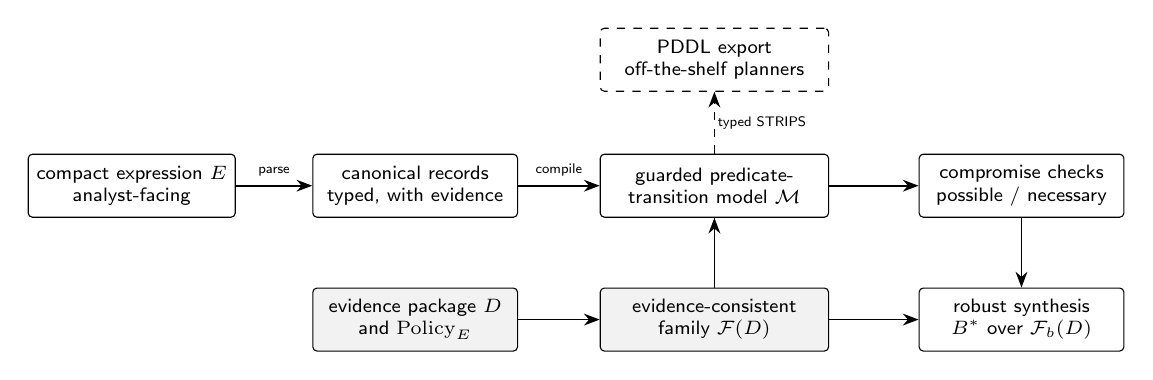
\begin{tikzpicture}[x=1cm,y=1cm]
\node[box, minimum width=2.6cm] (e) at (0,0) {compact expression $E$\\analyst-facing};
\node[box, minimum width=2.6cm] (c) at (3.6,0) {canonical records\\typed, with evidence};
\node[box, minimum width=2.9cm] (m) at (7.4,0) {guarded predicate-\\transition model $\mathcal{M}$};
\node[box, minimum width=2.6cm] (a) at (11.3,0) {compromise checks\\possible / necessary};
\node[box, minimum width=2.6cm] (s) at (11.3,-1.7) {robust synthesis\\$B^{*}$ over $\mathcal{F}_b(D)$};
\node[box, minimum width=2.6cm, fill=black!5] (d) at (3.6,-1.7) {evidence package $D$\\and $\mathrm{Policy}_E$};
\node[box, minimum width=2.9cm, fill=black!5] (f) at (7.4,-1.7) {evidence-consistent\\family $\mathcal{F}(D)$};
\node[box, minimum width=2.9cm, dashed] (p) at (7.4,1.6) {PDDL export\\off-the-shelf planners};
\draw[arr] (e) -- node[lbl,above=2pt]{parse} (c);
\draw[arr] (c) -- node[lbl,above=2pt]{compile} (m);
\draw[arr] (m) -- (a);
\draw[arr] (d) -- (f);
\draw[arr] (f) -- (s);
\draw[arr] (f.north) -- (m.south);
\draw[arr] (a) -- (s);
\draw[darr] (m) -- node[lbl,right]{typed STRIPS} (p);
\end{tikzpicture}
\caption{From analyst expression to analysis. Compilation must preserve the trace language (Proposition 1). Evidence determines which models are admissible; analyses quantify over that family. Because the compiled model is a typed STRIPS task, it can be exported to existing planners.}
\label{fig:pipeline}
\end{figure}

\begin{proposition}[Compiler correctness obligation]
A conformant compiler $\mathcal{C}$ satisfies $\mathrm{Traces}(\mathcal{C}(E),\St_0)=\Lang(E,\St_0)$ for every well-formed expression $E$ and initial state $\St_0$: it neither omits a licensed trace nor introduces an unlicensed one.
\end{proposition}
This is a specification that an implementation must discharge, not a theorem about all compilers. The proof strategy is structural induction on $E$: the atomic and identity cases follow from Equations~\eqref{eq:apply} and~\eqref{eq:sem1}; sequence from state threading; choice from union; repetition from the inductive unfolding; and concurrency from the restriction in Equation~\eqref{eq:par}. A reference implementation should make the obligation executable through round-trip tests and generated counterexamples.

\section{Evidence-Consistent Model Families}\label{sec:evidence}

Incident reconstruction rarely yields one certain model. Evidence may establish that an event occurred while leaving a guard ambiguous, or establish an initial fact without its origin. ACN therefore separates system semantics from epistemic admissibility.

\begin{definition}[Evidence-admission policy]
$\mathrm{Policy}_E$ is a declared rule set mapping an evidence object and the model field it supports to one of $\{\text{required},\text{admissible},\text{excluded}\}$. A policy may use status, provenance, support scope, time, and confidence (only when a method is declared). ACN does not prescribe a universal policy; the chosen policy is part of the research record.
\end{definition}

\begin{definition}[Evidence-consistent family]
For an evidence package $D$, the family contains every model and initial state whose atoms, initial facts, transitions, guards, effects, bindings, and temporal relations satisfy the constraints required or permitted by $\mathrm{Policy}_E$ and all type, domain, and invariant constraints:
\begin{equation}\label{eq:family}
\Fam(D)=\{(\Mod,\St_0)\ :\ \mathrm{EvidenceConsistent}(\Mod,\St_0,D,\mathrm{Policy}_E)\ \wedge\ \mathrm{DomainConsistent}(\Mod,\St_0)\}.
\end{equation}
\end{definition}
Uncertainty may concern an initial fact, a guard value, an effect, a binding, or temporal order, not only the presence of an edge. Evidence status changes which models are admissible, never transition probability or execution.

\section{Compromise, Complexity, and Robust Defensive Synthesis}\label{sec:synth}

\subsection{Prohibited goals, compromise, and modal compromise}

A prohibited goal $g$ is a finite set of well-typed atoms whose joint satisfaction constitutes the modeled failure; $G$ is a finite set of goals.

\begin{definition}[Model-relative compromise]
\begin{equation}\label{eq:comp}
\Comp(\Mod,\St_0,g)\iff \exists\pi\in T^{*}:\ \End(\St_0,\pi)\ \text{defined}\ \wedge\ \End(\St_0,\pi)\models g .
\end{equation}
\end{definition}
Traces range over all transitions of $\Mod$, including environment and legitimate-user transitions, because an attacker can benefit from them. This is the conservative choice. Incident replay may instead restrict traces to $\Lang(E,\St_0)$ for a reconstructed expression $E$; the restriction must be declared. The qualifier model-relative is mandatory: ACN establishes reachability or non-reachability only inside a declared model scope.

\begin{definition}[Possible and necessary compromise]
Over an evidence-consistent family,
\begin{align}
\mathrm{PossiblyCompromised}(D,g)&\iff \exists(\Mod,\St_0)\in\Fam(D):\ \Comp(\Mod,\St_0,g),\\
\mathrm{NecessarilyCompromised}(D,g)&\iff \forall(\Mod,\St_0)\in\Fam(D):\ \Comp(\Mod,\St_0,g).\label{eq:modal}
\end{align}
\end{definition}
The distinction answers two different analyst questions. Necessary compromise is what the evidence forces; possible compromise is what a defender must still rule out. Conformance Requirement~3 in Section~\ref{sec:conformance} depends on keeping the two apart.

\subsection{Complexity}\label{sec:complexity}

Because a ground ACN model is a typed STRIPS task, deciding $\Comp$ for one model is plan existence. For propositional STRIPS this is PSPACE-complete in general and NP-complete when plan length is polynomially bounded \cite{bylander1994}; these bounds are measured in the size of the ground model, which typed grounding can make exponentially larger than the compact expression. With finite domains the state space is finite, so reachability is decidable without any trace horizon; a horizon $L$ is needed only to enumerate $\Lang(E^{*},\St)$, and if one is imposed the guarantee weakens to $\Comp_L$, compromise within $L$ steps, which must then be stated. The synthesis problem below contains non-reachability as the special case of an empty control library, so it is PSPACE-hard in general. Under a polynomial horizon its decision version lies in $\Sigma_2^{p}$ (guess a bundle, then verify safety in every admissible model and task achievability), and it remains NP-hard because weighted hitting set and network interdiction embed as restricted cases \cite{nandi2016,bhuiyan2021}. Monotone attack-graph tools avoid these bounds by assuming facts are never deleted \cite{ammann2002,mulval}; ACN pays the cost in exchange for representing revocation and recovery.

\subsection{Controls as transformations}

\begin{definition}[Control]\label{def:control}
A control $\kappa$ is a deterministic transformation $\kappa(\Mod,\St_0)=(\Mod^{\kappa},\St_0^{\kappa})$. It may disable a transition, strengthen a guard, revoke trust, narrow authority, constrain a channel, block an effect, restore state, change an invariant, or restructure the model.
\end{definition}
A bundle $B=\langle\kappa_1,\dots,\kappa_m\rangle$ declares an application order and passes a conflict check:
\begin{equation}\label{eq:bundle}
\mathrm{ApplyControls}(B,(\Mod,\St_0))=\kappa_m\circ\cdots\circ\kappa_1(\Mod,\St_0)=(\Mod^{B},\St_0^{B}).
\end{equation}
If the controls commute on the relevant models, a canonical order may be used. The cost $J(B)$ is any declared bundle-level function and need not be additive.

\subsection{Robust task-preserving synthesis}

Pure attack-path minimization can select a control that destroys the business function. An authorized task is $q=(A_q,g_q)$: a set of authorized principals and a task goal. Let $T_{A_q}$ be the transitions whose executing principal is in $A_q$ or is an environment principal.
\begin{equation}\label{eq:utility}
U_Q(B;\Mod,\St_0)=\frac{1}{|Q|}\sum_{q\in Q}\mathbf{1}\big[\exists\pi\in T_{A_q}^{*}:\ \End(\St_0^{B},\pi)\models g_q\ \text{in}\ \Mod^{B}\big].
\end{equation}
Utility is defined per model because a control can break a task in one admissible model and not in another; weighted tasks are a direct generalization. Given a finite bounded family $\Fam_b(D)\subseteq\Fam(D)$, control bundles $\mathcal{B}$, goals $G$, and utility floor $\eta$, the robust synthesis problem is
\begin{equation}\label{eq:synth}
\begin{aligned}
B^{*}\in\arg\min_{B\in\mathcal{B}}\ & J(B)\\
\text{s.t.}\ \ & \forall(\Mod,\St_0)\in\Fam_b(D),\ \forall g\in G:\ \neg\Comp(\Mod^{B},\St_0^{B},g),\\
& \min_{(\Mod,\St_0)\in\Fam_b(D)} U_Q(B;\Mod,\St_0)\ge\eta ,
\end{aligned}
\end{equation}
with $B^{*}=\bot$ when no bundle is feasible. The utility constraint is worst-case over the same family as the safety constraint, so that a bundle cannot be accepted on the strength of a model in which it happens to preserve tasks.

\paragraph{Exact bounded profile.} Exact claims require a finite control library and bundle set, finite typed domains, finite task and goal suites, and a finite set of evidence alternatives. If $h$ independent binary evidence hypotheses are admitted, the family has at most $2^{h}$ members before domain consistency prunes it; a commuting $k$-control library has at most $2^{k}$ subsets. These are worst-case enumeration bounds, not efficiency guarantees. Larger instances may use counterexample-guided synthesis: solve against a working subset of models, search $\Fam_b(D)$ for a violating model and trace, add it, and repeat. Results based on sampling or heuristic pruning must be labeled approximate and cannot support the universal quantifier in Equation~\eqref{eq:synth}.

\section{Worked Example}\label{sec:example}

This section exercises every definition on one small model. Every value is computed by the reference checker \texttt{acn\_checks.py}, published with this paper. The example is a synthetic identity incident with no exploit content.

\paragraph{Evidence and family.} Logs show that attacker $A$ authenticated as user $U$ with a stolen password, that multi-factor authentication was not enforced for $U$, and that $A$ later read a protected database. How $A$ obtained administrative authority is unresolved: the evidence admits role assumption from $U$'s session (model $\Mod_1$) and use of an administrative key exposed in a repository (model $\Mod_2$). Under a policy that admits reconstructed escalation mechanisms, $\Fam_b(D)=\{\Mod_1,\Mod_2\}$. The two differ in one initial fact, $\mathrm{KEY}(\mathrm{admin})=\mathrm{exposed}$ with $\mathrm{KNOW}(A,\mathit{key})$, and one transition, $t_{2b}$.

\paragraph{Transitions.} With explicit values throughout:
{\small
\begin{align*}
t_1&:\ A\vdash[\mathrm{IA}\mid\mathrm{VALID\_CREDS}]\ \mathrm{IdP}(U):\ \mathrm{KNOW}(A,\mathit{cred}_U)\wedge\mathrm{MFA}(U)=\mathrm{off}\wedge\mathrm{SESSION}(A)=\mathrm{none}\\
&\qquad\Rightarrow\ \mathrm{SESSION}(A)=\mathrm{active}\\
t_2&:\ A\vdash[\mathrm{PE}\mid\mathrm{ASSUME}]\ \mathrm{IAM}(\mathrm{admin}):\ \mathrm{SESSION}(A)=\mathrm{active}\wedge\mathrm{ASSUMABLE}(\mathrm{admin})=\mathrm{true}\\
&\qquad\Rightarrow\ \mathrm{ROLESESS}(A)=\mathrm{active},\ \mathrm{AUTH}(A,\mathrm{admin})=\mathrm{active}\\
t_{2b}&:\ A\vdash[\mathrm{PE}\mid\mathrm{KEY}]\ \mathrm{IAM}(\mathrm{admin}):\ \mathrm{KEY}(\mathrm{admin})=\mathrm{exposed}\wedge\mathrm{KNOW}(A,\mathit{key})\\
&\qquad\Rightarrow\ \mathrm{AUTH}(A,\mathrm{admin})=\mathrm{active}\qquad(\Mod_2\ \text{only})\\
t_3&:\ A\vdash[\mathrm{COL}\mid\mathrm{READ}]\ \mathrm{DB}(\mathit{records}):\ \mathrm{AUTH}(A,\mathrm{admin})=\mathrm{active}\wedge\mathrm{READGATE}=\mathrm{open}\\
&\qquad\Rightarrow\ \mathrm{KNOW}(A,\mathit{records})\\
t_5&:\ A\vdash[\mathrm{STL}\mid\mathrm{LOGOUT}]\ \mathrm{IdP}(U):\ \mathrm{SESSION}(A)=\mathrm{active}\ \Rightarrow\ \mathrm{SESSION}(A)=\mathrm{none}
\end{align*}}
Each value update deletes the previous value of the same atom. The invariant $\Inv$ adds value exclusivity and $\mathrm{ROLESESS}(x)=\mathrm{active}\Rightarrow\mathrm{SESSION}(x)=\mathrm{active}$. Legitimate transitions let $U$ log in (with MFA if enforced, using a registered device) and assume the admin role, and let the backup service read the database when $\mathrm{READGATE}=\mathrm{open}$.

\paragraph{Semantics in action.} In $\St_0$ of $\Mod_1$, $t_1$ is enabled. After $t_1$ and $t_2$, $t_5$ is \emph{not} enabled: its guard holds, but the successor would leave a role session without a login session, violating $\Inv$. This is the invariant-timing rule of Equation~\eqref{eq:enabled} rejecting a state that a guard-only check would accept. The trace $t_1t_2t_3$ is valid. After $t_2$, the attacker read $t_3$ and the backup read are independent under Equation~\eqref{eq:indep}, so they may be composed with $\parallel$. After $t_1$ alone, $t_2$ and $t_5$ are both enabled but not independent: logging out disables role assumption.

\paragraph{Compromise.} With goal $g=\{\mathrm{KNOW}(A,\mathit{records})\}$, both models are compromised, with shortest witnesses $t_1t_2t_3$ in $\Mod_1$ and $t_{2b}t_3$ in $\Mod_2$. The incident is therefore necessarily compromised. After control $k_1$ alone it is possibly but not necessarily compromised.

\paragraph{Controls and tasks.} The control library is $k_1$ enforce MFA (cost 2), $k_2$ revoke role assumability (cost 1), $k_3$ rotate and vault the exposed key (cost 1), and $k_4$ require break-glass approval for every database read (cost 4). The controls set independent initial values, so they commute. The task suite is $q_1$: $U$ can obtain admin authority for maintenance, and $q_2$: the backup service completes its read. Table~\ref{tab:example} lists representative bundles out of all 16 evaluated.

\begin{table}[t]
\centering\small
\caption{Selected bundles from the worked example. All 16 subsets are evaluated exactly by the reference checker.}\label{tab:example}
\begin{tabular}{@{}lccccl@{}}
\toprule
Bundle $B$ & $J(B)$ & Safe in $\Mod_1$ & Safe in $\Mod_2$ & $\min U_Q$ & Note \\
\midrule
$\emptyset$ & 0 & no & no & 1.0 & necessarily compromised \\
$\{k_1\}$ & 2 & yes & no & 1.0 & optimal if only $\Mod_1$ is considered \\
$\{k_2\}$ & 1 & yes & no & 0.5 & breaks $q_1$ \\
$\{k_3\}$ & 1 & no & no & 1.0 & \\
$\{k_4\}$ & 4 & yes & yes & 0.5 & breaks $q_2$ \\
$\{k_2,k_3\}$ & 2 & yes & yes & 0.5 & attack-only optimum \\
$\{k_1,k_3\}$ & 3 & yes & yes & 1.0 & robust optimum at $\eta=1$ \\
\bottomrule
\end{tabular}
\end{table}

\paragraph{Results.} Three findings follow, each computed exactly.
\begin{enumerate}[leftmargin=1.5em,itemsep=1pt]
\item \emph{Robust synthesis.} With $\eta=1$, $B^{*}=\{k_1,k_3\}$ at cost 3.
\item \emph{Single-model analysis fails.} Restricting the analysis to $\Mod_1$, the most direct reading of the logs, selects $\{k_1\}$ at cost 2. That bundle leaves $\Mod_2$ compromised: the attacker escalates through the exposed key. Quantifying over the family is what exposes the gap.
\item \emph{Attack-only minimization breaks the business.} Ignoring utility ($\eta=0$) selects $\{k_2,k_3\}$ at cost 2, which blocks both attack paths but removes $U$'s legitimate maintenance access, so $\min U_Q=0.5$. The same bundle is the correct answer if the operator declares $\eta=0.5$, which makes the business tradeoff an explicit, recorded decision rather than a side effect of the optimizer.
\end{enumerate}

\begin{figure}[t]
\centering
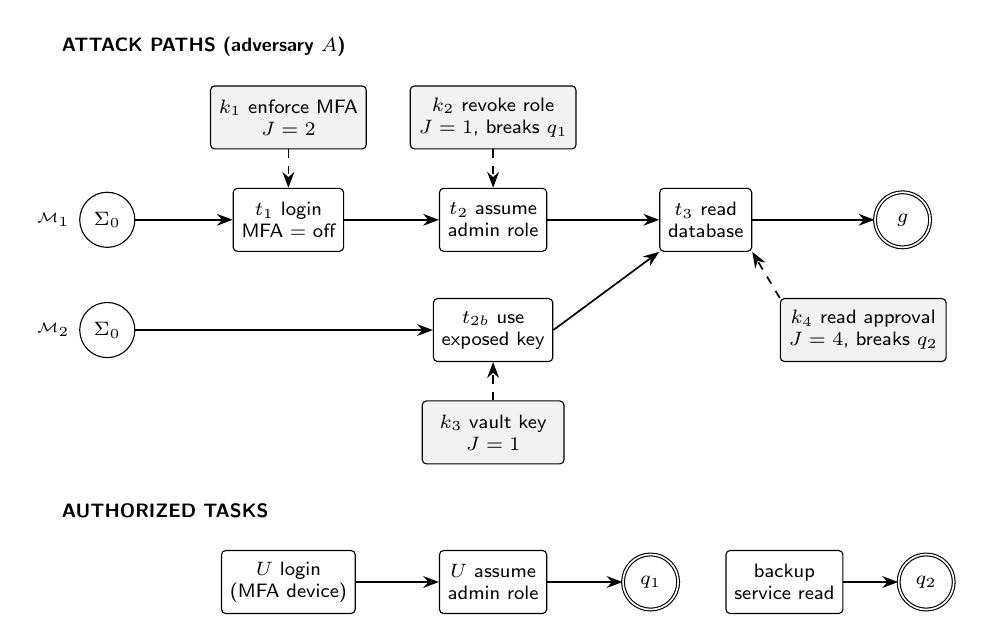
\begin{tikzpicture}[x=1cm,y=1cm]
\node[font=\sffamily\scriptsize\bfseries, anchor=west] at (-0.7,5.1) {ATTACK PATHS (adversary $A$)};
\node[box, minimum width=1.8cm, fill=black!5] (k1) at (2.3,4.2) {$k_1$ enforce MFA\\$J=2$};
\node[box, minimum width=1.8cm, fill=black!5] (k2) at (4.9,4.2) {$k_2$ revoke role\\$J=1$, breaks $q_1$};
\node[st] (s1) at (0,2.9) {$\Sigma_0$};
\node[font=\sffamily\tiny, anchor=east] at (s1.west) {$\mathcal{M}_1$};
\node[box] (t1) at (2.3,2.9) {$t_1$ login\\MFA = off};
\node[box] (t2) at (4.9,2.9) {$t_2$ assume\\admin role};
\node[box] (t3) at (7.6,2.9) {$t_3$ read\\database};
\node[goal] (g) at (10.1,2.9) {$g$};
\node[st] (s2) at (0,1.5) {$\Sigma_0$};
\node[font=\sffamily\tiny, anchor=east] at (s2.west) {$\mathcal{M}_2$};
\node[box] (t2b) at (4.9,1.5) {$t_{2b}$ use\\exposed key};
\node[box, minimum width=1.8cm, fill=black!5] (k3) at (4.9,0.2) {$k_3$ vault key\\$J=1$};
\node[box, minimum width=1.8cm, fill=black!5] (k4) at (9.6,1.5) {$k_4$ read approval\\$J=4$, breaks $q_2$};
\draw[arr] (s1) -- (t1); \draw[arr] (t1) -- (t2); \draw[arr] (t2) -- (t3); \draw[arr] (t3) -- (g);
\draw[arr] (s2) -- (t2b); \draw[arr] (t2b.east) -- (t3.south west);
\draw[darr] (k1) -- (t1); \draw[darr] (k2) -- (t2); \draw[darr] (k3) -- (t2b); \draw[darr] (k4.north west) -- (t3.south east);
\node[font=\sffamily\scriptsize\bfseries, anchor=west] at (-0.7,-0.8) {AUTHORIZED TASKS};
\node[box] (u1) at (2.3,-1.7) {$U$ login\\(MFA device)};
\node[box] (u2) at (4.9,-1.7) {$U$ assume\\admin role};
\node[goal] (gq1) at (6.9,-1.7) {$q_1$};
\node[box] (b1) at (8.6,-1.7) {backup\\service read};
\node[goal] (gq2) at (10.4,-1.7) {$q_2$};
\draw[arr] (u1) -- (u2); \draw[arr] (u2) -- (gq1); \draw[arr] (b1) -- (gq2);
\end{tikzpicture}
\caption{Worked example. Solid arrows are transitions; dashed arrows show which transition each control disables. $k_2$ also blocks the legitimate role assumption in $q_1$, and $k_4$ also blocks the backup read in $q_2$. $\{k_1,k_3\}$ blocks every attack path in both admissible models and preserves both tasks; $\{k_1\}$ alone leaves the $\Mod_2$ path open; $\{k_2,k_3\}$ is cheaper but breaks $q_1$.}
\label{fig:example}
\end{figure}

\paragraph{Excess authority.} Section~\ref{sec:authority} is exercised on an agent holding
\[H=\{\mathrm{read}(/\mathrm{data}/*),\ \mathrm{send}(*@\mathrm{corp}),\ \mathrm{delete}(/\mathrm{tmp}/*),\ \mathrm{share}(/\mathrm{data}/\mathrm{report})\}\]
with weights $3,2,4,1$, and a task with two incomparable minimal realizations,
\[R_1=\{\mathrm{read}(/\mathrm{data}/\mathrm{report}),\ \mathrm{send}(\mathrm{boss}@\mathrm{corp})\},\qquad R_2=\{\mathrm{read}(/\mathrm{data}/\mathrm{report}),\ \mathrm{share}(/\mathrm{data}/\mathrm{report})\}.\]
Plain set inclusion reports both realizations infeasible, because neither $R_1\subseteq H$ nor $R_2\subseteq H$, although $H$ clearly covers both. With the subsumption order both are feasible, the excess is 5 for $R_1$ and 6 for $R_2$, and $[\mathrm{EA}_{\min},\mathrm{EA}_{\max}]=[5,6]$.

\section{Cross-Domain Stress Tests}\label{sec:stress}

These examples test whether one typed guard and effect semantics covers materially different domains. They are semantic stress tests, not empirical demonstrations, and they avoid exploit-specific detail.

\subsection{Mobile reachability: Manic}\label{sec:manic}

ThreatFabric's August 2026 analysis of the Manic Android malware reports that when direct command-and-control connectivity is unavailable, infected devices queue encrypted data and relay it through nearby infected devices over Wi-Fi Direct, Bluetooth RFCOMM, or Bluetooth Low Energy, with a default limit of four relay hops carried in the relay metadata \cite{manic}. The graph-theoretic observation is modest:
\begin{equation}
\neg\mathrm{Direct}(v,C_2)\ \not\Rightarrow\ \neg\mathrm{Reachable}(v,C_2).
\end{equation}
The state that makes it operational is queued data, a nearby infected peer, an alternate radio path, and a remaining hop budget. One relay hop from device $v$ to peer $p$ is
\begin{equation}
\begin{aligned}
&w\vdash[\mathrm{EXF}\mid\mathrm{RELAY}]\ \mathrm{PEER}(d)@\mathrm{RADIO}:\\
&\qquad \mathrm{HOLDS}(v,d)\wedge\mathrm{NEAR}(v,p)\wedge\mathrm{INFECTED}(p)\wedge\mathrm{HOPS}(d)=k\wedge k<4\\
&\qquad\Rightarrow\ \mathrm{HOLDS}(p,d),\ \mathrm{HOPS}(d)=k{+}1\ \evsep\ \mathrm{R},
\end{aligned}
\end{equation}
where $w$ denotes the malware instance, so as not to overload the model symbol $\Mod$, and the update to $\mathrm{HOPS}$ deletes the previous value. Exfiltration completes with an upload transition guarded by $\mathrm{HOLDS}(p,d)\wedge\mathrm{ONLINE}(p)$. The full behavior is the bounded expression $\mathrm{RELAY}^{\le 4}\rightarrow\mathrm{UPLOAD}$. The example shows why removing direct Internet reachability from one device does not remove every modeled path, and why the hop budget belongs in the state rather than in prose.

\subsection{Ransomware as a trace schema}

A ransomware operation is not one universal linear theorem. With IA initial access, EXE execution, PE privilege escalation, PER persistence, DIS discovery, CA credential access, LM lateral movement, DIMP defense impairment, COL collection, and EXF exfiltration,
\begin{equation}
R=\mathrm{IA}\rightarrow\mathrm{EXE}\rightarrow(\mathrm{PE}\oplus\mathbb{1})\rightarrow\mathrm{PER}^{*}\rightarrow\mathrm{DIS}\rightarrow(\mathrm{CA}\rightarrow\mathrm{LM})^{*}\rightarrow\mathrm{DIMP}^{*}\rightarrow(\mathrm{COL}\rightarrow\mathrm{EXF})^{*}\rightarrow\mathrm{IMP}_{\mathrm{encrypt}}
\end{equation}
is a trace schema, not a definition. Each realized label expands to typed transitions with concrete guards and effects. The DIMP label corresponds to the Defense Impairment tactic that ATT\&CK v19 split from the former Defense Evasion tactic, alongside Stealth \cite{attack}; such labels remain external metadata.

\subsection{API authorization failure}

Absence, denial, and non-enforcement must be distinguished. A broken object-level authorization transition states all three explicitly:
\begin{equation}
\begin{aligned}
&A\vdash[\mathrm{COL}\mid\mathrm{ACCESS}]\ \mathrm{API}(r_j)@\mathrm{HTTPS}:\\
&\qquad \mathrm{AUTHN}(A)\wedge\mathrm{AUTHZ}(A,j)=\mathrm{denied}\wedge\mathrm{ENFORCED}(\mathrm{API},j)=\mathrm{false}\\
&\qquad\Rightarrow\ \mathrm{KNOW}(A,r_j)\ \evsep\ \mathrm{R}.
\end{aligned}
\end{equation}
A secure API with $\mathrm{ENFORCED}(\mathrm{API},j)=\mathrm{true}$ rejects the same denied decision. Not being authorized is not sufficient for disclosure, and unknown is never read as false.

\subsection{Cloud identity}

Cloud incidents often move through delegated identity rather than host traversal:
\begin{equation}
\begin{aligned}
&A\vdash[\mathrm{PE}\mid\mathrm{ABUSE}]\ \mathrm{IAM}(r)@\mathrm{STS}:\\
&\qquad \mathrm{TOKEN}(A,t)=\mathrm{valid}\wedge\mathrm{ASSUME\_ALLOWED}(t,r)\\
&\qquad\Rightarrow\ \mathrm{AUTH}(A,r)=\mathrm{active}\ \evsep\ \mathrm{R}.
\end{aligned}
\end{equation}
The ACN effect is the authority state that changed; ATT\&CK labels remain classification metadata.

\subsection{Cyber-physical process state}

Industrial systems need process-state predicates and external safety invariants:
\begin{equation}
\begin{aligned}
&A\vdash[\mathrm{IPC}\mid\mathrm{STATE}]\ \mathrm{PLC}(\mathit{sp})@\mathrm{OT}:\\
&\qquad \mathrm{CONTROL}(A,\mathrm{EWS})\wedge\mathrm{WRITE\_ALLOWED}(\mathrm{EWS},\mathrm{PLC})\wedge\mathrm{INTERLOCK}(\mathrm{PLC})=\mathrm{bypassed}\\
&\qquad\Rightarrow\ \mathrm{MODE}(\mathrm{PLC})=\mathrm{unsafe}\ \evsep\ \mathrm{R}.
\end{aligned}
\end{equation}
This is a discrete security abstraction, not a plant model. $\Inv$ may reference invariants verified by continuous-control or hybrid-system analysis, and a hardware interlock is a control that prevents the unsafe successor.

\section{AI-Agent Extension}\label{sec:ai}

AI agents stress the calculus because security-relevant state is neither purely host based nor purely identity based. The model must separate attacker-influenced context from deterministic policy, model-selected actions from authorized effects, and user authority from authority delegated to an agent. Existing work addresses each of these \cite{taskshield,camel,progent,authgraph,xiong2026,skillguard}; ACN's role is to express them in one transition semantics.
\begin{equation}
\St^{\mathrm{AI}}=\langle\St;\ X,\ H,\ \mathcal{O},\ \mathcal{R},\ \Pi,\ \mathcal{E}\rangle,
\end{equation}
where $X$ is context and decision state, $H$ the agent's enforceable capability set, $\mathcal{O}$ the enabled tool operations, $\mathcal{R}$ the reachable resources, $\Pi$ deterministic policy enforced outside generative inference, and $\mathcal{E}$ the permitted external effects. $\Pi$ changes only through an explicit policy transition or control. The agent appears in transitions as executing principal $\mathit{ag}$, with the attacker as influencing principal where influence is modeled (Definition~\ref{def:atomic}).

\subsection{Capabilities and subsumption}\label{sec:authority}

A capability is parameterized: $c=\langle \mathit{op},\mathit{scope},\mathit{constraints},\mathit{effect},\mathit{validity}\rangle$. Because scopes nest, authority comparison needs an order rather than set equality. Define $c\sqsubseteq c'$ ($c'$ covers $c$) when both have the same operation and effect class, $\mathit{scope}(c)\subseteq\mathit{scope}(c')$, every argument satisfying $\mathit{constraints}(c)$ satisfies $\mathit{constraints}(c')$, and $\mathit{validity}(c)\subseteq\mathit{validity}(c')$. Lift it to sets:
\begin{equation}
R\sqsubseteq H\iff \forall c\in R\ \exists c'\in H:\ c\sqsubseteq c',\qquad \mathrm{Used}(H,R)=\{c'\in H:\ \exists c\in R,\ c\sqsubseteq c'\}.
\end{equation}
The delegation invariant is $H_{\mathrm{agent}}(t)\sqsubseteq H_{\mathrm{deleg}}(\mathit{user},\mathit{ctx},t)$, where $H_{\mathrm{deleg}}=\mathrm{Delegable}(\Pi_t,\mathit{user},\mathit{ctx},t)$. Plain set inclusion is wrong here: an agent holding $\mathrm{read}(/\mathrm{data}/*)$ covers a required $\mathrm{read}(/\mathrm{data}/\mathrm{report})$, but $\{\mathrm{read}(/\mathrm{data}/\mathrm{report})\}\not\subseteq\{\mathrm{read}(/\mathrm{data}/*)\}$. Section~\ref{sec:example} shows inclusion reporting a covered task as infeasible.

\subsection{Minimal sufficient authority and excess authority}

$\mathrm{Req}(q,t)$ is the family of minimal capability sets sufficient for authorized task $q$ at time $t$ under the declared platform, policy, and workflow model, minimal with respect to $\sqsubseteq$. The feasible realizations are
\begin{equation}
\mathrm{Req}_H(q,t)=\{R\in\mathrm{Req}(q,t):\ R\sqsubseteq H_{\mathrm{agent}}(t)\}.
\end{equation}
If an authorized plan $p$ is selected with requirement $R_p$, the plan-relative Authority Gap is the set of held capabilities that the plan never uses:
\begin{equation}
\Delta H_p(t)=H_{\mathrm{agent}}(t)\setminus\mathrm{Used}(H_{\mathrm{agent}}(t),R_p).
\end{equation}
When several incomparable minimal realizations exist and no plan has been selected, ACN reports an interval rather than inventing a canonical requirement. With a declared nonnegative exposure weight $w$ and documented calibration,
\begin{equation}\label{eq:ea}
\mathrm{EA}_{\min}(q,t)=\min_{R\in\mathrm{Req}_H(q,t)}\sum_{c'\in H\setminus\mathrm{Used}(H,R)} w(c'),\qquad
\mathrm{EA}_{\max}(q,t)=\max_{R\in\mathrm{Req}_H(q,t)}\sum_{c'\in H\setminus\mathrm{Used}(H,R)} w(c').
\end{equation}
Both are undefined when $\mathrm{Req}_H(q,t)=\emptyset$, meaning current authority is insufficient. A runtime policy that must choose one realization before planning declares its own deterministic selection rule, which becomes part of $\Pi$ and of the research record. The measure counts unused capabilities. Over-breadth of a used capability, such as holding $\mathrm{read}(/\mathrm{data}/*)$ to read one file, requires a declared scope measure and is left as an explicit extension. $\mathrm{EA}_{\min}$ and $\mathrm{EA}_{\max}$ measure removable excess authority under stated weights; they are not breach probabilities.

\subsection{From influence to a prohibited effect}

Retrieved data is not assumed to become a system instruction. The weaker security-relevant predicate is that attacker-controlled content influences decision state. Unless telemetry supports the causal link, the step is reconstructed:
\begin{equation}
\begin{aligned}
&A\vdash[\mathrm{AIS}\mid\mathrm{INJECT}]\ \mathit{ctx}(X)@\mathrm{CONTEXT}:\\
&\qquad \mathrm{RETRIEVED}(\mathit{ag},d_m)\wedge\mathrm{ATTACKER\_CTRL}(d_m)\wedge\mathrm{ACTIVE}(\mathit{ag},d_m)\\
&\qquad\Rightarrow\ \mathrm{INFL}(A,X_{\mathit{ag}})\ \evsep\ \mathrm{R}.
\end{aligned}
\end{equation}
The agent then acts as executing principal under the attacker's influence:
\begin{align}
\mathit{ag}\triangleleft A&\vdash[\mathrm{EXE}\mid\mathrm{INVOKE}]\ T(\vec x)@\mathrm{TOOL}:\ \mathrm{INFL}(A,X_{\mathit{ag}})\wedge\{\mathrm{invoke}(T,\vec x)\}\sqsubseteq H_t\notag\\
&\qquad\wedge\ \mathrm{ALLOW}(\Pi_t,\mathrm{invoke}(T,\vec x))\ \Rightarrow\ \mathrm{INVOKED}(T,\vec x)\ \evsep\ \mathrm{R}\\
\mathit{ag}\triangleleft A&\vdash[\mathrm{DIS}\mid\mathrm{READ}]\ \mathrm{search}(s)@\mathrm{TOOL}:\ \mathrm{INVOKED}(\mathrm{search},s)\wedge\mathit{secret}\in\mathcal{R}_t(s)\notag\\
&\qquad\Rightarrow\ \mathrm{KNOW}(\mathit{ag},\mathit{secret})\ \evsep\ \mathrm{R}\\
\mathit{ag}\triangleleft A&\vdash[\mathrm{EXF}\mid\mathrm{SEND}]\ \mathrm{send}(d_A)@\mathrm{EGRESS}:\ \mathrm{KNOW}(\mathit{ag},\mathit{secret})\notag\\
&\qquad\wedge\ \{\mathrm{send}(d_A)\}\sqsubseteq H_t
\wedge d_A\in\mathcal{E}_t\wedge\mathrm{ALLOW}(\Pi_t,\mathrm{send}(d_A))\notag\\
&\qquad\Rightarrow\ \mathrm{POSSESS}(A,\mathit{secret})\ \evsep\ \mathrm{R}
\end{align}
The second step is the first under the binding $\theta=\{T\mapsto\mathrm{search},\ \vec x\mapsto s\}$. The sequence separates context influence, authorized invocation, agent knowledge, and attacker possession. The agent learning a secret does not imply exfiltration; the final effect requires a separately enabled sink transition with parameter-scoped authority, policy permission, and an allowed egress destination. The dual principals record that the agent executed every step and that the attacker influenced it, which is the distinction between influence and authority that recent agent-security work makes central \cite{authgraph,camel}.

\begin{figure}[t]
\centering
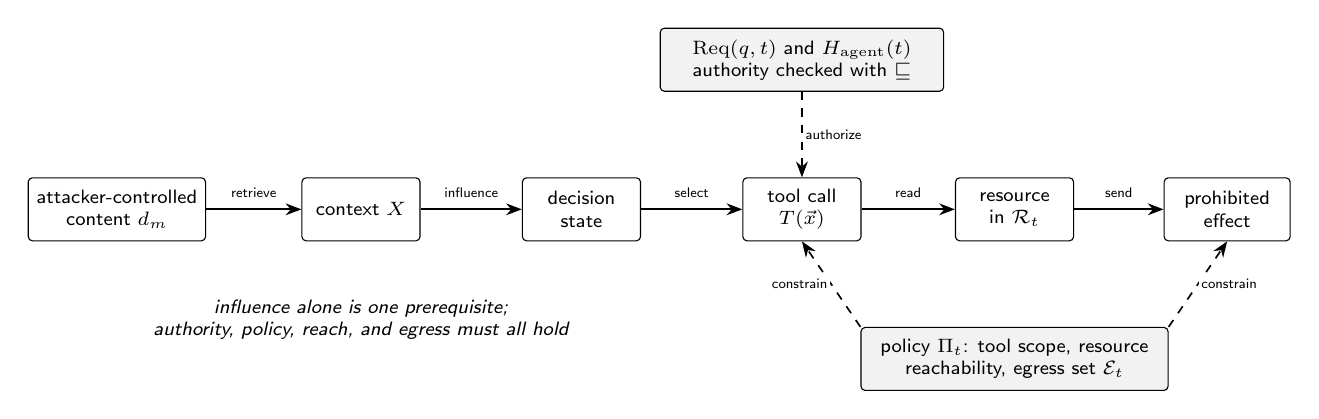
\begin{tikzpicture}[x=1cm,y=1cm]
\node[box, minimum width=1.9cm] (d) at (0,0) {attacker-controlled\\content $d_m$};
\node[box, minimum width=1.5cm] (x) at (3.1,0) {context $X$};
\node[box, minimum width=1.5cm] (ds) at (5.9,0) {decision\\state};
\node[box, minimum width=1.5cm] (tc) at (8.7,0) {tool call\\$T(\vec x)$};
\node[box, minimum width=1.5cm] (rq) at (11.4,0) {resource\\in $\mathcal{R}_t$};
\node[box, minimum width=1.6cm] (pe) at (14.1,0) {prohibited\\effect};
\draw[arr] (d) -- node[lbl,above=3pt]{retrieve} (x);
\draw[arr] (x) -- node[lbl,above=3pt]{influence} (ds);
\draw[arr] (ds) -- node[lbl,above=3pt]{select} (tc);
\draw[arr] (tc) -- node[lbl,above=3pt]{read} (rq);
\draw[arr] (rq) -- node[lbl,above=3pt]{send} (pe);
\node[box, minimum width=3.6cm, fill=black!5] (req) at (8.7,1.9) {$\mathrm{Req}(q,t)$ and $H_{\mathrm{agent}}(t)$\\authority checked with $\sqsubseteq$};
\node[box, minimum width=3.9cm, fill=black!5] (pol) at (11.4,-1.9) {policy $\Pi_t$: tool scope, resource\\reachability, egress set $\mathcal{E}_t$};
\draw[darr] (req) -- node[lbl,right]{authorize} (tc);
\draw[darr] (pol.north west) -- node[lbl,left]{constrain} (tc.south);
\draw[darr] (pol.north east) -- node[lbl,right]{constrain} (pe.south);
\node[capn] at (3.1,-1.4) {influence alone is one prerequisite;\\authority, policy, reach, and egress must all hold};
\end{tikzpicture}
\caption{AI-agent extension. Context influence is one prerequisite among several. Parameter-scoped authority, deterministic policy, resource reachability, and egress must all license a path before a prohibited effect is reachable, and each is a point where a control can act.}
\label{fig:ai}
\end{figure}

\subsection{Containment as control synthesis}

Agent controls act at source admission, context isolation, tool and action allowlists, parameter scope, delegated authority, resource reachability, deterministic policy, and egress. ACN does not require prompt injection to be impossible. It requires the bounded model to have no enabled trace from attacker influence to a prohibited goal while preserving declared task utility, which is Equation~\eqref{eq:synth} applied to agent controls.

\section{Falsifiable Hypotheses and Evaluation}\label{sec:eval}

Internal consistency is not empirical validation, and no results are reported here. Baselines are unstructured narrative analysis, ATT\&CK-only tagging, and an established formal method suited to the experiment, such as MAL, attack-defense trees, or a PDDL planning encoding.

\begin{table}[t]
\centering\small
\caption{Evaluation program. These are falsifiable hypotheses, not findings.}\label{tab:eval}
\begin{tabularx}{\textwidth}{@{}l X X@{}}
\toprule
Hypothesis & Claim under test & Primary measurements \\
\midrule
H1 causal validity & ACN encodings expose seeded missing prerequisites and contradictory effects more reliably than narrative analysis. & Pre-registered defect-detection F1; precision, recall, time. \\
H2 analyst agreement & Independent analysts produce compatible canonical encodings from the same evidence. & Field-specific Krippendorff $\alpha$, predicate-set Jaccard, semantic trace comparison. \\
H3 compiler correctness & Compact to canonical to executable preserves $\Lang(E,\St_0)$. & Round-trip conformance; property-based tests; counterexample count. \\
H4 cross-domain adequacy & One core grammar encodes mobile, API, cloud, ransomware, AI, and ICS cases without overloading. & Required extensions; invalid coercions; coverage. \\
H5 defense quality & Robust task-preserving synthesis reduces prohibited reachability with less task loss than attack-only and single-model baselines. & Residual compromise over $\Fam_b(D)$; worst-case $U_Q$; cost; runtime. Agent instances on AgentDojo \cite{agentdojo}. \\
H6 readability & Compact ACN improves comprehension of guards, effects, and evidence at acceptable learning cost. & Accuracy and time; error rate; workload; prior formal-methods experience controlled. \\
\bottomrule
\end{tabularx}
\end{table}

The corpus should cover ransomware, cloud identity compromise, API authorization failure, mobile device takeover, supply-chain compromise, business email compromise, an AI-agent prompt-injection case, and an ICS process-manipulation case. Each case uses a frozen evidence package, a narrative baseline, external mappings, and a blinded encoding phase. Public reporting, first-party telemetry, and reconstruction must remain distinguishable. Analysts encode independently; primary metrics, sample size, and power analysis are pre-registered; disagreement about evidence status is separated from disagreement about predicate choice. Solver experiments publish the bounded profile: domains, horizon if any, evidence alternatives, model count, bundle count, goals, tasks, exact or approximate method, configuration, and timeout. Because ACN compiles to STRIPS, H5 should include an off-the-shelf planner as a reachability baseline.

ACN should be narrowed or rejected if the core grammar repeatedly needs ad hoc semantics for ordinary cases, analysts cannot reach acceptable agreement after training, the compiler cannot preserve trace semantics, extensions routinely overload predicates, or synthesis shows no benefit over simpler baselines at comparable effort.

\section{Conformance Conditions}\label{sec:conformance}

\begin{table}[t]
\centering\small
\caption{Minimum machine-checkable conformance conditions.}\label{tab:conf}
\begin{tabularx}{\textwidth}{@{}l X@{}}
\toprule
Check & Requirement \\
\midrule
Type correctness & Every value, argument, capability, target, object, channel, and binding satisfies its declared sort. \\
Ground execution & Executable transitions have no unbound variables; substitutions are type-preserving and consistent. \\
Explicit values & Guards never use negation-as-failure; negative states are explicit values with provenance. \\
Guard and invariant validity & $\Pre$ holds and the full delete-then-add successor satisfies $\Inv$ before enablement. \\
Effect consistency & $\Add\cap\Del=\emptyset$; valued effects respect exclusivity. \\
Evidence provenance & Every transition and every initial atom resolves to a source or rationale; confidence has a declared method. \\
Principals & Executing and influencing principals are distinguished wherever they differ. \\
Temporal consistency & Ordering does not contradict timestamps or declared causal constraints. \\
Concurrency & Concurrent transitions satisfy Equation~\eqref{eq:indep} wherever concurrency is claimed. \\
Control bundles & Each bundle declares an order or proven commutativity and passes conflict validation. \\
Compiler correctness & Compact to canonical to executable preserves $\Lang(E,\St_0)$. \\
Robustness scope & Every containment claim states $\Fam_b(D)$, goals, bundles, tasks, $\eta$, horizon if any, and exact or approximate status. \\
\bottomrule
\end{tabularx}
\end{table}

\paragraph{Requirement 1 (No hidden prerequisite).} Every guard atom consumed by a valid trace is present in $\St_0$ with an evidence object, or was produced by an earlier transition and not removed before use.

\paragraph{Requirement 2 (Control relevance).} A control is relevant to a goal only if its transformation changes the enablement or effects of an executable trace to that goal, changes the initial valuation so the trace becomes invalid, or changes the goal under explicitly modeled recovery semantics.

\paragraph{Requirement 3 (Evidence transparency).} Tightening $\mathrm{Policy}_E$ to exclude reconstructed hypotheses must not change a conclusion advertised as observed-only. If it does, the conclusion depended on reconstruction and is mislabeled. In modal terms, an observed-only claim of compromise must be a necessary compromise under the observed-only family.

\section{Open Research, Reproducibility, and Release Boundary}

This paper is released as independent open-source research, open to implementation, criticism, counterexample construction, and empirical testing. The reference checker published with it implements valued states, invariants, enablement, application, trace execution, independence, exact reachability, possible and necessary compromise, controls, robust synthesis, and subsumption-aware excess authority, and it reproduces every value in Section~\ref{sec:example}. It is a minimal executable semantics, not the full parser and solver described in Section~\ref{sec:roadmap}.

The research profile is defensive: incident reconstruction, threat modeling, authorized testing, formal-methods research, education, and control comparison. Public artifacts should model adversary behavior only at the level needed to validate state semantics, without novel exploit code, credential-theft implementations, destructive commands, evasion recipes, or step-by-step intrusion procedures. Synthetic fixtures, like the worked example, are preferred whenever a real artifact would add abuse value without scientific value. This is a release policy, not a claim that a notation can prevent misuse.

\section{Limitations}

A well-formed model can create false rigor if mistaken for proof about the world; scope and evidence remain explicit for that reason. State explosion is unavoidable as identities, tokens, resources, time, and hypotheses are instantiated, and the complexity bounds of Section~\ref{sec:complexity} apply. Boolean and finite-valued atoms are a deliberate simplification: belief, stochastic behavior, continuous processes, and temporal authorization need epistemic, probabilistic, temporal, or hybrid extensions. Intent and mechanism vocabularies drift as external frameworks change, which is why mappings stay metadata. Reconstructed hypotheses remain subject to analyst bias, and the family construction makes that bias visible rather than removing it. The excess-authority measure counts unused capabilities but not over-breadth of used ones. Finally, no multi-analyst study, benchmarked compiler, solver evaluation, or usability experiment is reported; claims of improved accuracy, usability, or defensive effectiveness remain hypotheses.

\section{Roadmap}\label{sec:roadmap}

The next milestone is a public specification package: grammar, type declarations, canonical schema, evidence-policy schema, invariant rules, and conformance tests. The second is a parser and validator that round-trips compact expressions and canonical records and exports ground models to PDDL, so that existing planners serve as reachability engines. The third is an independently encoded corpus with documented adjudication, followed by bounded synthesis experiments. If ACN can map to ATT\&CK for taxonomy, STIX for exchange, D3FEND for countermeasures, MAL and planning formalisms for reasoning, and policy engines for enforcement without unacceptable semantic loss, it functions as a bridge rather than another competing encyclopedia. If interoperability or analyst agreement cannot be demonstrated, the project should be narrowed.

\section{Conclusion}

Attack Calculus does not claim that state machines, precondition-effect attack languages, attack graphs, planning, least privilege, or interdiction are new. Its proposed contribution is their disciplined integration into an analyst-facing intermediate representation: a typed transition that binds principals, intent, mechanism, valued guards, effects, and evidence; a canonical model with non-monotone updates and a known place in the complexity landscape; evidence-consistent families with possible and necessary compromise; and synthesis that eliminates modeled prohibited outcomes in every admissible model while preserving authorized work in the worst admissible model. The worked example shows the two failures this design exists to prevent: a defense that is optimal for the most likely reading of the evidence and wrong for an admissible alternative, and a defense that is cheapest against the attacker and breaks the business. Whether the representation earns its keep is an empirical question, and this release makes it precise enough to test.

\section*{Availability}

The paper source and the reference checker are published at \url{https://github.com/codethor0/attack-calculus}. Corrections, counterexamples, and implementations are welcome.

\small
\begin{thebibliography}{99}\setlength{\itemsep}{1pt}
\bibitem{cuppens2000} F.~Cuppens and R.~Ortalo, ``LAMBDA: A Language to Model a Database for Detection of Attacks,'' in \emph{Recent Advances in Intrusion Detection (RAID)}, LNCS 1907, pp.~197--216, 2000.
\bibitem{templeton2000} S.~J. Templeton and K.~Levitt, ``A Requires/Provides Model for Computer Attacks,'' in \emph{Proc. New Security Paradigms Workshop}, pp.~31--38, 2000.
\bibitem{statl} S.~T. Eckmann, G.~Vigna, and R.~A. Kemmerer, ``STATL: An Attack Language for State-Based Intrusion Detection,'' \emph{Journal of Computer Security} 10(1--2), 71--103, 2002.
\bibitem{ning2002} P.~Ning, Y.~Cui, and D.~S. Reeves, ``Constructing Attack Scenarios through Correlation of Intrusion Alerts,'' in \emph{Proc. ACM CCS}, pp.~245--254, 2002.
\bibitem{sheyner2002} O.~Sheyner, J.~Haines, S.~Jha, R.~Lippmann, and J.~M. Wing, ``Automated Generation and Analysis of Attack Graphs,'' in \emph{Proc. IEEE Symposium on Security and Privacy}, pp.~273--284, 2002.
\bibitem{ammann2002} P.~Ammann, D.~Wijesekera, and S.~Kaushik, ``Scalable, Graph-Based Network Vulnerability Analysis,'' in \emph{Proc. ACM CCS}, pp.~217--224, 2002.
\bibitem{mulval} X.~Ou, S.~Govindavajhala, and A.~W. Appel, ``MulVAL: A Logic-based Network Security Analyzer,'' in \emph{Proc. USENIX Security Symposium}, 2005.
\bibitem{adtrees} B.~Kordy, S.~Mauw, S.~Radomirovi\'c, and P.~Schweitzer, ``Attack-Defense Trees,'' \emph{Journal of Logic and Computation} 24(1), 55--87, 2014.
\bibitem{mal} W.~Wide\l{} et~al., ``The Meta Attack Language: A Formal Description,'' \emph{Computers \& Security} 130, 103284, 2023.
\bibitem{konsta2024} A.-M. Konsta, A.~Lluch Lafuente, B.~Spiga, and N.~Dragoni, ``Survey: Automatic Generation of Attack Trees and Attack Graphs,'' \emph{Computers \& Security} 137, 103602, 2024.
\bibitem{boddy2005} M.~Boddy, J.~Gohde, T.~Haigh, and S.~Harp, ``Course of Action Generation for Cyber Security Using Classical Planning,'' in \emph{Proc. ICAPS}, pp.~12--21, 2005.
\bibitem{obes2010} J.~Lucangeli Obes, C.~Sarraute, and G.~Richarte, ``Attack Planning in the Real World,'' in \emph{Proc. AAAI Workshop on Intelligent Security (SecArt)}, 2010. arXiv:1306.4044.
\bibitem{hoffmann2015} J.~Hoffmann, ``Simulated Penetration Testing: From `Dijkstra' to `Turing Test++','' in \emph{Proc. ICAPS}, 2015.
\bibitem{strips} R.~E. Fikes and N.~J. Nilsson, ``STRIPS: A New Approach to the Application of Theorem Proving to Problem Solving,'' \emph{Artificial Intelligence} 2(3--4), 189--208, 1971.
\bibitem{pddl} D.~McDermott et~al., ``PDDL: The Planning Domain Definition Language,'' Technical Report CVC TR-98-003, Yale Center for Computational Vision and Control, 1998.
\bibitem{bylander1994} T.~Bylander, ``The Computational Complexity of Propositional STRIPS Planning,'' \emph{Artificial Intelligence} 69(1--2), 165--204, 1994.
\bibitem{genrich1981} H.~J. Genrich and K.~Lautenbach, ``System Modelling with High-Level Petri Nets,'' \emph{Theoretical Computer Science} 13(1), 109--135, 1981.
\bibitem{mazurkiewicz1987} A.~Mazurkiewicz, ``Trace Theory,'' in \emph{Petri Nets: Applications and Relationships to Other Models of Concurrency}, LNCS 255, pp.~279--324, 1987.
\bibitem{godefroid1996} P.~Godefroid, \emph{Partial-Order Methods for the Verification of Concurrent Systems}, LNCS 1032, Springer, 1996.
\bibitem{attack} MITRE ATT\&CK, ``Updates: April 2026'' (v19) and ``Updates: August 2026'' (v19.2), The MITRE Corporation, 2026. \url{https://attack.mitre.org/resources/updates/}
\bibitem{d3fend} P.~E. Kaloroumakis and M.~J. Smith, ``Toward a Knowledge Graph of Cybersecurity Countermeasures,'' The MITRE Corporation, 2021; MITRE D3FEND. \url{https://d3fend.mitre.org/}
\bibitem{stix} OASIS Cyber Threat Intelligence Technical Committee, ``STIX Version 2.1,'' OASIS Standard, 2021.
\bibitem{nandi2016} A.~K. Nandi, H.~R. Medal, and S.~Vadlamani, ``Interdicting Attack Graphs to Protect Organizations from Cyber Attacks: A Bi-Level Defender-Attacker Model,'' \emph{Computers \& Operations Research} 75, 118--131, 2016.
\bibitem{bhuiyan2021} T.~H. Bhuiyan, H.~R. Medal, A.~K. Nandi, and M.~Halappanavar, ``Risk-Averse Bi-Level Stochastic Network Interdiction Model for Cyber-Security Risk Management,'' \emph{International Journal of Critical Infrastructure Protection} 32, 100408, 2021.
\bibitem{miam} T.~Thor, ``Mission-Invariant Architecture Morphing: Service-Graph Reconfiguration Against Post-Access Reconnaissance, with Cryptographic Epoch Isolation and Mission-Domain State Continuity,'' Zenodo, 2026. \url{https://doi.org/10.5281/zenodo.23001045}
\bibitem{openai2025} OpenAI, ``Understanding Prompt Injections: A Frontier Security Challenge,'' November 2025.
\bibitem{toolhijacker} J.~Shi, Z.~Yuan, G.~Tie, P.~Zhou, N.~Z. Gong, and L.~Sun, ``Prompt Injection Attack to Tool Selection in LLM Agents,'' arXiv:2504.19793, 2025.
\bibitem{taskshield} F.~Jia, T.~Wu, X.~Qin, and A.~Squicciarini, ``The Task Shield: Enforcing Task Alignment to Defend Against Indirect Prompt Injection in LLM Agents,'' in \emph{Proc. ACL}, 2025.
\bibitem{camel} E.~Debenedetti et~al., ``Defeating Prompt Injections by Design,'' arXiv:2503.18813, 2025.
\bibitem{progent} T.~Shi et~al., ``Progent: Programmable Privilege Control for LLM Agents,'' arXiv:2504.11703, 2025.
\bibitem{openai2026} OpenAI, ``Designing AI Agents to Resist Prompt Injection,'' March 2026.
\bibitem{microsoft2026} Microsoft Security, ``Least Privilege for AI Agents: Identity, Access, and Tool Binding,'' Microsoft Security Blog, July 16, 2026.
\bibitem{authgraph} P.~Wang, Y.~Li, and Y.~Tian, ``Aligning Provenance with Authorization: A Dual-Graph Defense for LLM Agents,'' arXiv:2605.26497, 2026.
\bibitem{xiong2026} W.~Xiong, R.~Karanjai, Y.~Lu, W.~Shi, and L.~Xu, ``Reachability-Based Capability Confinement for LLM Agents under Indirect Prompt Injection,'' arXiv:2608.30041, 2026.
\bibitem{skillguard} S.~Pan, X.~Sun, T.~Zhang, D.~Liao, M.~Si, and Z.~Xing, ``SkillGuard: A Permission Framework for Agent Skills,'' arXiv:2606.03024v1, 2026. (Revised in v2 as ``SkillGuard: A Permission-Centric Framework for Agent Skill Security.'')
\bibitem{agentdojo} E.~Debenedetti et~al., ``AgentDojo: A Dynamic Environment to Evaluate Prompt Injection Attacks and Defenses for LLM Agents,'' arXiv:2406.13352, 2024.
\bibitem{prov} W3C, ``PROV-DM: The PROV Data Model,'' W3C Recommendation, 2013.
\bibitem{manic} ThreatFabric Mobile Threat Intelligence, ``Manic: Blend between Banking Malware and Spyware,'' August 20, 2026.
\end{thebibliography}
\normalsize

\appendix
\renewcommand{\thesection}{Appendix \Alph{section}.}
\titleformat{\section}{\normalfont\large\bfseries}{\thesection}{0.5em}{}

\section{Core Grammar and Precedence}

\begin{center}\small
\begin{tabular}{@{}l@{}}
$\mathit{Atomic}\ ::=\ \mathit{principal}\ [\,\triangleleft\ \mathit{principal}\,]\ \vdash\ [\,\mathit{intent}\mid\mathit{mechanism}\,]\ \mathit{target}(\mathit{object})\ @\ \mathit{channel}$\\
$\hspace{5.2em} :\ \Pre\ \Rightarrow\ (\Add,\Del)\ \evsep\ \mathit{evidence}$\\[3pt]
$\mathit{Expr}\ ::=\ \mathit{Choice}$\\
$\mathit{Choice}\ ::=\ \mathit{Parallel}\ \{\ \oplus\ \mathit{Parallel}\ \}$\\
$\mathit{Parallel}\ ::=\ \mathit{Sequence}\ \{\ \parallel\ \mathit{Sequence}\ \}$\\
$\mathit{Sequence}\ ::=\ \mathit{Repeat}\ \{\ \rightarrow\ \mathit{Repeat}\ \}$\\
$\mathit{Repeat}\ ::=\ \mathit{Primary}\ [\ ^{*}\ \mid\ ^{\le k}\ ]$\\
$\mathit{Primary}\ ::=\ \mathbb{1}\mid\mathit{Atomic}\mid(\,\mathit{Expr}\,)$
\end{tabular}
\end{center}
Parentheses bind explicitly; repetition binds most tightly, then sequence, then concurrency, then choice. Star is finite Kleene closure; $^{\le k}$ is bounded repetition. Executable transitions are ground after type-preserving substitution.

\section{Canonical Record Example}\label{app:record}

\begin{small}
\begin{verbatim}
transition_id: api-bola-read-001
executing_principal: A
influencing_principal: null
intent: COL
mechanism: ACCESS
target: API
object: record_j
channel: HTTPS
preconditions:
  - AUTHN(A)=true
  - AUTHZ(A,j)=denied
  - ENFORCED(API,j)=false
add_effects:
  - KNOW(A,record_j)=true
delete_effects: []
evidence:
  status: R
  confidence: null
  method: null
  provenance: synthetic-example
  support: [guard, add_effect]
initial_atom_evidence:
  - atom: ENFORCED(API,j)=false
    status: R
    provenance: synthetic-example
framework_mappings: []
\end{verbatim}
\end{small}

\section{Notation}

\begin{center}\small
\begin{tabular}{@{}ll@{}}
\toprule
Symbol & Meaning \\
\midrule
$\Sigma$, $\Sigma_0$ & Well-typed state; initial state \\
$\Gamma$ & Domain invariants, including value exclusivity, checked on the full successor \\
$\Delta$ & Type environment \\
$\tau$; $a\triangleleft b$ & Ground transition; executing principal $a$ influenced by $b$ \\
$\Pre,\Add,\Del$ & Valued guards; additive and destructive effects \\
$e$ & Evidence object (transitions and initial atoms) \\
$\mathbb{1}$; $\rightarrow,\parallel,\oplus,{}^{*},{}^{\le k}$ & Identity; sequence, concurrency, choice, repetition, bounded repetition \\
$\Lang(E,\Sigma)$ & Finite trace language of $E$ from $\Sigma$ \\
$\mathcal{M}$ & Guarded predicate-transition model \\
$\mathcal{F}(D)$, $\mathcal{F}_b(D)$ & Evidence-consistent family; bounded family \\
$G$, $g$; $Q$, $q$ & Prohibited goals; authorized tasks \\
$B$, $J(B)$, $\eta$ & Control bundle, cost, utility floor \\
$X,H,\mathcal{O},\mathcal{R},\Pi,\mathcal{E}$ & Agent context, capabilities, tool operations, resources, policy, permitted effects \\
$c\sqsubseteq c'$ & Capability subsumption \\
$\mathrm{EA}_{\min},\mathrm{EA}_{\max}$ & Excess-authority interval \\
\bottomrule
\end{tabular}
\end{center}

\end{document}
